%%==================================================================%%
%% Author : Abascal Fern�ndez, Patricia                             %%
%%          S�nchez Barreiro, Pablo                                 %%
%% Version: 1.0, 14/02/2013                                         %%                                                                                    %%                                                                  %%
%% Memoria del Proyecto Fin de Carrera                              %%
%% Archivo ra�z                                                     %%
%%==================================================================%%

\documentclass[a4paper,11pt]{itsas_pfc}

%=====================================================================%
%                       My imported packages                          %
%=====================================================================%
\usepackage[latin1]{inputenc}
\usepackage{longtable}
\usepackage{array}
\usepackage{url}
\usepackage{amsfonts}
\usepackage[spanish,activeacute]{babel} 
% File with main configuration
%
% Potentially useful packages (rec = recommended, opt = optional)
%
\usepackage{fancyhdr}          % (rec)  allows for the customization of various header/footer parameters
% \usepackage{courier}         % (opt)  uses that font by default
% \usepackage{setspace}        % (opt)  allows for inter-line space changing
\usepackage{longtable}         % (opt)  allows for multi-page tables
% \usepackage{lscape}          % (opt)  allows for the use of \landscape
\usepackage{color}             % (opt)  various color-related commands (like \color)
\usepackage{rotating}          % (opt)  allows for PS and EPS rotation
% \usepackage{textcomp}        % (opt)  allows for euro sign, with \texteuro
\usepackage[spanish]{minitoc}           % (opt)  allows for per-chapter tables of contents
\usepackage{epsf}              % (opt)  allow for certain EPS manipulations
%\usepackage[utf8x]{inputenc}  % (opt)  allows for some text editors to show \'{a} as �, and so on.
\usepackage[absolute]{textpos} % (rec)  allows for arbitrary positioning of text (required for default cover page)
% \usepackage{srcltx}            % (opt)  allows to pass from .dvi back to the .tex
%
% Margin settings. Uncomment and modify if you know what you are doing. Note
% that a further 1 inch is added to the margins given here. The given values are
% the default ones for A4 paper, and itsas_pfc.cls style.
%
\setlength{\oddsidemargin}{0.3in}     % left margin for odd (right) pages
\setlength{\evensidemargin}{0.3in}    % left margin for even (left) pages
\setlength{\textwidth}{6in}        % width of the text body

%
% Recommended to improve the automatic positioning of figures.
% (taken from http://dcwww.camp.dtu.dk/~schiotz/comp/LatexTips/LatexTips.html#captfont)
%
\renewcommand{\topfraction}{0.85}
\renewcommand{\textfraction}{0.1}
\renewcommand{\floatpagefraction}{0.75}

%
% Space between top border of page and where text begins (headers go there)
% LaTeX complains if using package fancyhdr and headheight is below 15pt
%
\headheight 15pt

%
% For the textpos package (used when making the cover page)
%
\setlength{\TPHorizModule}{\paperwidth}
\setlength{\TPVertModule}{\paperheight}
\newcommand{\tb}[4]{\begin{textblock}{#1}[0.5,0.5](#2,#3)\begin{center}#4\end{center}\end{textblock}}

%
% You can define your commands here
%
% \newcommand{cmd}[args]{def}
% cmd  = command to define (e.g. \water)
% args = number of arguments
% def  = the definition, where #1, #2,... is the 1st, 2nd... argument
%
% E.g.:
%
% \newcommand{\water}[1]{H\ensuremath{_#1}O}
%
%
%
% Each time we write "\water{33}", the output will be: "H33O" (with 33 subscripted)
%

%
% You can teach LaTeX how to hypenize some words here
% E.g.: to cut "gnomonly" only where dashed (-).
%
\hyphenation{gno-mon-ly}

%
% Start book with Roman-numbered pages
% Will be changed to arabics later on
%
\pagenumbering{Roman}


% File with some names
%
% This file has a list of internal names (variables) of LaTeX,
% of which you can change the value. For example, you can make
% chapters read "Section" instead of "Chapter".
%
\renewcommand\bibname{References}                 % thus Bibliography will read "References"
%\renewcommand{\tablename}{xxx}                   % name below each table (xxx 1: bla-bla-bla)
%\renewcommand{\figurename}{xxx}                  % name below each figure (xxx 1: bla-bla-bla)
%\renewcommand{\listtablename}{yyy}               % name for table of tables
%\renewcommand{\listfigurename}{yyy}              % name for table of figures


%=====================================================================%
%                           Authoring's details                       %
%=====================================================================%
\newcommand{\myname}{Patricia Abascal Fern�ndez}  % name of author
\newcommand{\myboss}{Pablo S�nchez Barreiro} % name of supervisor
\newcommand{\thesistitle}{Desarrollo de un entorno dirigido por modelos para el desarrollo de l�neas de productos software para la plataforma .NET}

\newcommand{\englishtitle}{Development of a model-driven development enviroment for software product lines on the .NET platform}
												  % work title
\newcommand{\worktype}{Proyecto Fin de Carrera}   % work type
\newcommand{\logo}{images/uc.eps}            % logo file (e.g. for the cover)

%=====================================================================%
%                     Definition of my own commands                   %
%=====================================================================%
\newcommand{\nota}[1]{\color{red}$\ll$#1$\gg$\color{black}}
\newcommand{\imp}[1]{{\small{\sf #1}}}
\newcommand{\stereotype}[1]{$\ll${\small{\sf #1}}$\gg$}
\newcommand{\todo}[1]{\color{red}$\ll$TODO: #1$\gg$\color{black}}

\setcounter{minitocdepth}{1}

\begin{document}

% Cover page
% %
% This file produces the first page of the PFC/Thesis, featuring
% the title, your name, supervisor's name and so forth.
%
% Most, if not all, content in this page is included via commands
% (e.g. \thesistitle) that have been defined in Config/pfc_options.tex
%
% Edit to your liking.
%

\thispagestyle{empty} % don't print neither page number nor headers nor footers.

%
% Use \tb to place the various items in the page. Usage:
%
% \tb{w}{h}{v}{t}
%
% where:
%
% w = paragraph width of text box (1.0 = page width)
% h = horizontal position of the center of text box (0.0 = left, 1.0 = right)
% v = vertical position of the center of text box (0.0 = top, 1.0 = bottom)
% t = text to put inside text box
%
\tb{0.8}{0.50}{0.100}{\large FACULTAD DE CIENCIAS}
\tb{0.8}{0.50}{0.130}{\Large UNIVERSIDAD DE CANTABRIA}
\tb{0.8}{0.50}{0.250}{
	
\includegraphics[width=0.30\columnwidth]{images/ingInformatica.eps} \ \ \ \ \
}
\tb{0.8}{0.50}{0.390}{\LARGE \worktype}    % whether this is a PFC or a Thesis
\tb{0.8}{0.50}{0.500}{\Huge \thesistitle}  % title of the work
\tb{0.8}{0.50}{0.600}{\LARGE (\englishtitle)}  % title of the work
\tb{0.8}{0.50}{0.700}{\Large Para acceder al T�tulo de \\
					  INGENIERO EN INFORM�TICA}   % the name of the supervisor
\tb{0.2}{0.70}{0.850}{\begin{tabular}{r}
\Large Autor: Alejandro P�rez Ruiz \\
\Large Julio 2011 \\
\end{tabular}}

\ \clearpage                       % end page here
\thispagestyle{empty} \ \clearpage % blank page


% \begin{tabular}{p{.15\textwidth}p{.50\textwidth}p{.15\textwidth}}
	\includegraphics[width=\linewidth]{\logo} & 
	\begin{center}FACULTAD DE CIENCIAS\end{center} & \\
\end{tabular}

\vspace{-15pt}

\begin{center}
INGENIER�A EN INFORM�TICA
\end{center}

\begin{center}
CALIFICACI�N DEL PROYECTO FIN DE CARRERA
\end{center}

\begin{tabular}{p{0.25\textwidth}p{0.75\textwidth}}
Realizado por:    & \myname \\ 
Director del PFC: & \myboss \\
T�tulo:           & \thesistitle  \\   
Title:            & \englishtitle \\  
\end{tabular}


Presentado a examen el d�a: 

\begin{center}
para acceder al T�tulo de \\ 
INGENIERO EN INFORM�TICA
\end{center}

\underline{Composici�n del Tribunal:} \\

\begin{tabular}{ll}
Presidente (Apellidos, Nombre): & \\
Secretario (Apellidos, Nombre): & \\
Vocal (Apellidos, Nombre): & \\
Vocal (Apellidos, Nombre): & \\
Vocal (Apellidos, Nombre): & \\
\end{tabular}

\ \\

Este Tribunal ha resuelto otorgar la calificaci�n de: ......................................

\begin{center}
\begin{tabular}{cc}
& \\
& \\
& \\
\ \ \ \ \ \ \ \ \ \ \ \
Fdo.: El Presidente 
\ \ \ \ \ \ \ \ \ \ \ \ &  
\ \ \ \ \ \ \ \ \ \ \ \
Fdo.: El Secretario  
\ \ \ \ \ \ \ \ \ \ \ \ \\
& \\
& \\
& \\
Fdo.: Vocal \ \ \ \ \ \          &         Fdo.: Vocal \ \ \ \ \ \ \\
& \\
& \\
& \\
Fdo.: Vocal \ \ \ \ \ \          &         Fdo.: El Director del PFC \ \ \ \ \ \  \\
\end{tabular}
\end{center}

\thispagestyle{empty} \



% reset page numbering
% Use \cdpchapter for all chapters that start in a "right side" page,
% AND have no number (e.g. Acknowledgements):
\newcommand{\cdpchapter}[1]{\cleardoublepage\chapter*{#1}}

% Start counting pages from 1 again:
\setcounter{page}{1}


% acknowledgement
% \cdpchapter{Agradecimientos}

A toda mi familia por haberme apoyado durante todos estos a�os de estudio,y en especial a mis padres que siempre han estado conmigo en los buenos y malos momentos.\\\\

A mi director Pablo S�nchez por brindarme la oportunidad de realizar este proyecto, guiarme en todo su desarrollo y sobretodo, contestarme a un sinf�n de preguntas.\\\\

A todos mis compa�eros de clase que han estado junto a m� y que tan buenos momentos me han hecho pasar dentro y fuera de clase.\\\\

A todos los profesores de Ingenier�a Inform�tica de la Universidad de Cantabria por transmitirnos sus conocimientos.\\\\


 % acknowledgements

% Preface
%%%==================================================================%%
%% Author : Abascal Fern�ndez, Patricia                             %%
%%          S�nchez Barreiro, Pablo                                 %%
%% Version: 1.3, 18/06/2013                                         %%                                                                                    %%                                                                  %%
%% Memoria del Proyecto Fin de Carrera                              %%
%% Archivo ra�z                                                     %%
%%==================================================================%%

\cdpchapter{Resumen}
Dentro del Departamento de Matem�ticas, Estad�stica y Computaci�n se han desarrollado con anterioridad una serie de t�cnicas para la implementaci�n y configuraci�n de l�neas de productos software para la plataforma .NET bas�ndose en las clases parciales de C\#. Dichas t�cnicas se condensan en el denominado \emph{Slicer Pattern}. No obstante, la aplicaci�n de dicho patr�n de forma manual implica una serie de tareas manuales y repetitivas.

El objetivo de presente proyecto fin de carrera es desarrollar una serie de generadores de c�digo que permitan automatizar la aplicaci�n del \emph{Slicer Pattern}. Ello reducir�a los tiempos de desarrollo; y , por tanto, el coste. Adem�s, al automatizarse el proceso se evita la introducci�n de errores debidos a la intervenci�n humana. Esto contribuye a aumentar la calidad del producto final y a reducir los tiempos y costes de desarrollo; ya que el tiempo necesario para detectar y corregir estos potenciales errores desaparece.

Para alcanzar dicho objetivo, este proyecto fin de carrera ha desarrollado una serie de generadores de c�digo que transforman modelos de dise�o, en UML 2.0, de una l�nea de productos software en una implementaci�n en C\# basada en el \emph{Slicer Pattern}. Dichos generadores de c�digo se han implementado usando EGL (\emph{Epsilon Generation Language}), el lenguaje de transformaci�n modelo a c�digo de la suite de herramientas para la manipulaci�n de modelos \emph{Epsilon}.

\paragraph{Palabras Clave} \ \\

L�nea de Productos Software, Generaci�n de C�digo, Desarrollo Software Orientado a Caracter�sticas, Clases Parciales C\#, Patr�n Slicer, .NET, Epsilon, Te.NET, TENTE.



   % preface

% Toc
% \dominitoc        % each chapter has its ToC (requires package "minitoc")
\tableofcontents  % insert ToC here
\listoffigures    % insert List of Figures here (optional)
\listoftables     % insert List of Tables here (optional)

\cleardoublepage






\pagestyle{fancy}                                % choose this heading style (recommended)
\fancyhf{}                                       % delete previous style, to then redefine it
\fancyhead[LE,RO]{\textbf{\thepage}}             % Header: page number in boldface

\fancyhead[RE]{\nouppercase{\leftmark}}          % Header: upper-level info (Chapter) to the right (R) of even (E)
                                                 % pages, preventing ALLCAPS (which would be the default)

\fancyhead[LO]{\nouppercase{\rightmark}}         % Header: include info about lower level (Section) to the left (L)
                                                 % of odd (O) pages, preventing ALLCAPS

\renewcommand{\headrulewidth}{0.5pt}             % Header: underline the header (set to "0pt" if unwanted)
\renewcommand{\footrulewidth}{0pt}               % Footer: underline footer (set to "0pt" if unwanted)


\setcounter{page}{1}   % start numbering pages from 1 on (again)
\pagenumbering{arabic} % use arabic numbers, again

% Use \tocchapter instead of \chapter, to make use of
% nicely formatted chapter front pages:
\newcommand{\tocchapter}[1]{\cleardoublepage\chapter{#1}\minitoc\newpage}

% \newcommand{\chapterheader}[1]{\cleardoublepage\chapter{#1}}
\newcommand{\chapterheader}[2]{\cleardoublepage\chapter[#2]{#1}} 

\newcommand{\chaptertoc}{\minitoc}


% Cap�tulo 1: Introducci�n
% %%==================================================================%%
%% Author : Abascal Fern�ndez, Patricia                             %%
%%          S�nchez Barreiro, Pablo                                 %%
%% Version: 2.1, 14/06/2013                                         %%                                                                                    %%                                                                  %%
%% Memoria del Proyecto Fin de Carrera                              %%
%% Archivo ra�z                                                     %%
%%==================================================================%%

\chapterheader{Introducci�n}{Introducci�n}
\label{chap:introduction}

Este cap�tulo sirve de introducci�n a la presente Memoria de Proyecto Fin de Carrera. Para ello, en primer lugar se describe el contexto general donde se enmarca dicho proyecto y que da lugar al mismo. Se describe luego, a grandes rasgos, el proyecto para la metodolog�a Te.Net, proyecto general de amplio alcance donde se inscribe el presente proyecto. A continuaci�n, se exponen los objetivos principales del proyecto. Por �ltimo, se describe c�mo se estructura el presente documento.

\chaptertoc

\section{Contexto del Proyecto}
\label{sec:intr:introduction}

%%==================================================================%%
%% Author : Abascal Fern�ndez, Patricia                             %%
%%          S�nchez Barreiro, Pablo                                 %%
%% Version: 1.2, 23/04/2013                                         %%                                                                                    %%                                                                  %%
%% Memoria del Proyecto Fin de Carrera                              %%
%% Introducci�n                                                     %%
%%==================================================================%%

El principal objetivo de este Proyecto de Fin de Carrera es implementar un conjunto de generadores de c�digo que permitan transformar modelos UML orientados a caracter�sticas en c�digo C\#. Para dar soporte a la orientaci�n a caracter�sticas a nivel de c�digo C\#, se utilizar� el patr�n de dise�o
\emph{Slicer}. Dicho patr�n fue espec�ficamente para tal prop�sito como parte de otro Proyecto Fin de Carrera presentado en esta misma Facultad~\cite{}. 

La \emph{orientaci�n a caracter�sticas}~\cite{} tiene como objetivo  encapsular porciones coherentes de la funcionalidad proporcionadas por una aplicaci�n en m�dulos independientes llamados \emph{caracter�sticas}. La orientaci�n a caracter�sticas eleva el nivel al cual se agrupa la funcionalidad de un sistema del concepto de clase al concepto de \emph{conjunto} o \emph{familia de clases}, las cuales se a�aden o eliminan de una aplicaci�n como un todo. 

De esta forma, podemos obtener productos con funcionalidades ligeramente diferentes mediante la simple incorporaci�n o eliminaci�n de m�dulos representando caracter�sticas. 

Lo que convierte la obtenci�n de diferentes versiones de una misma aplicaci�n combinando diferentes conjuntos de caracter�sticas en una tarea sencilla. Los \emph{dise�os orientados a caracter�sticas} deben asegurar que el resultado de la composici�n de un conjunto de caracter�sticas produce como resultado una aplicaci�n correcta y segura.


La orientaci�n a caracter�sticas~\cite{} se utiliza frecuentemente como mecanismo de dise�o e implementaci�n de las conocidas como \emph{L�neas de Productos Sw}~\cite{}.

El objetivo de una \emph{L�neas de Productos Sw}~\cite{} es ... \todo{Copiar la definici�n del proyecto de Alejandro o de Daniel}.

%%===================================================================%%
%% NOTA(Pablo): Establecer relaci�n entre ambos paradigmas           %%
%%===================================================================%%

Este Proyecto Fin de Carrera se enmarca dentro un proyecto general y m�s ambicioso

Dichos generadores de c�digo se integrar�an en una metodolog�a m�s amplia para el desarrollo de \emph{L�neas de Productos Software}~\cite{}, denominada Te.Net.


es integrar dichos generadores en la metodolog�a de desarrollo de \emph{L�neas de Productos Software}~\cite{} denominada TE.NET, una versi�n para la plataforma .NET de la metodolog�a TENTE~\cite{}. A continuaci�n intentaremos introducir de forma breve al lector en estos conceptos.



Dada la cantidad de terminolog�a novedosa contenida en la descripci�n del proyecto, procedemos a describir brevemente la historia precedente a la gestaci�n del mismo.


%%===================================================================%%
%% NOTA(Pablo): Esto se mueve mejor a antecedentes                   %%
%%===================================================================%%
%%
%% El uso de las l�neas de producto software permite la reducci�n
%% de costes de desarrollo por la reutilizaci�n de la tecnolog�a en
%% los distintos sistemas, a mayor cantidad de productos a desarrollar
%% mayor rentabilidad respecto a los sistemas creados individualmente.
%% Ofrece alta calidad en el producto resultante porque se realizan
%% pruebas de los componentes de la plataforma en diferentes tipos
%% de producto para ayudar a detectar y corregir errores. Reduce el
%% tiempo de creaci�n debido a la reutilizaci�n de los componentes ya
%% existentes para cada nuevo producto y reduce tambi�n el esfuerzo
%% requerido por el mantenimiento ya que cuando se cambia algo de un
%% componente de la plataforma, ese cambio se propaga a todos los
%% componentes que lo empleen, y de esta forma se reduce el esfuerzo
%% de aprender c�mo funciona cada elemento individualmente.
%%
%% En contraposici�n a la flexibilidad que ofrece el desarrollo de
%% software individual, espec�fico para cliente pero que supone grandes
%%  costes, las l�neas de producto software delimitan las variaciones
%% de sus productos a un conjunto prefijado y optimizan, por tanto, los
%% procesos para dichas variaciones.
%%
%%
%% La l�nea de productos software se puede extrapolar a otros �mbitos de
%% producci�n. Un ejemplo cl�sico de l�nea de productos es la fabricaci�n
%% de autom�viles, donde se ofrece al cliente un modelo base al cual puede
%% a�adir aquellos extras que as� desee, personalizando el veh�culo y
%%  adapt�ndolo a sus necesidades. De esta forma partiendo del mismo modelo
%% y de unas variaciones adicionales preestablecidas, y dise�adas de tal
%% forma que se adaptan perfectamente al modelo seleccionado, se puede
%% obtener gran cantidad de variaciones en el modelo final de manera
%% autom�tica.

En el �mbito del desarrollo software, las empresas ya no se centran en la creaci�n de un producto espec�fico para un cliente (por ejemplo, dise�ar y construir un portal para la Universidad de Cantabria), sino en un domino (por ejemplo, dise�ar y construir un portal para universidades). Los principales desaf�os a los que se enfrentan las empresas son: delimitar dicho dominio, identificar las distintas variaciones que se van a permitir y desarrollar la infraestructura que permita realizar los productos a bajo coste sin reducir la calidad.


%%%%%%%%%%%% Metodolog�as de desarrollo de l�neas de productos software %%%%%%%%%%%%

El proceso de desarrollo de la l�nea de productos software se divide en dos procesos \cite{pohl:2010}: Ingenier�a de Dominio e Ingenier�a de la Aplicaci�n. Por un lado la \emph{Ingenier�a del Dominio} se encarga de la construcci�n de la plataforma mediante la delimitaci�n del conjunto de aplicaciones para las que est� creada, adem�s de definir y construir qu� caracter�sticas ser�n reusables y cuales espec�ficas para cada uno de los productos que se desean fabricar.

Por otra parte, la \emph{Ingenier�a de la Aplicaci�n} se encarga de la creaci�n de los productos para clientes concretos. Partiendo de la plataforma creada en la fase de Ingenier�a de Dominio, y reutilizando tantos componentes como fuera necesario, se crea una especializaci�n del producto base acorde a los requisitos del cliente.


%%%%%%%%%%%% Clases parciales y patr�n Slicer %%%%%%%%%%%%
Tal como se ha descrito al inicio de este apartado, el objetivo del presente Proyecto Fin de Carrera consiste en el desarrollo e implementaci�n de unos generadores de c�digo que permitan la tranformaci�n del dise�o de los modelos en una implementaci�n en c�digo C\# de dichos dise�os, para ello se usar�n las prestaciones que ofrecen el uso de las clases parciales del lenguaje C\# basadas en el patr�n Slicer.

Las \emph{clases parciales} permiten a los desarrolladores fragmentar la implementaci�n de una clase en un conjunto de ficheros, cada uno de los cuales contiene una porci�n, o incremento, de una funcionalidad de la clase. Sin embargo, no ofrecen ning�n mecanismo para agrupar o encapsular caracter�sticas, por lo que no es posible ocultar clases y m�todos que pertenecen a una caracter�stica espec�fica de aquellas clases y m�todos que pertenecen a caracter�sticas independientes. Adem�s, permiten a�adir nuevos atributos y m�todos a existentes clases parciales pero no permite sobreescribir o extender m�todos ya existentes.

Para solventar dichos problemas, el profesor Pablo S�nchez, dentro del Departamento de Matem�ticas, Estad�stica y Computaci�n, ha desarrollado un patr�n de dise�o llamado \emph{Patr�n Slicer} \cite{perez:2011} que parte de la siguiente idea: todos los problemas que se pretenden solucionar tienen origen en el hecho de no poner tener m�todos con el mismo nombre en distintas clases parciales, hay que evitar dicha situaci�n. Estos fragmentos de clases parciales, son combinados en tiempo de compilaci�n para crear una �nica clase que auna todas las caracter�sticas seleccionadas inicialmente por el cliente.

Por ejemplo, supongamos que un cliente quiere un veh�culo con varias caracter�sticas adicionales entre las que se encuentran: aire acondicionado, sensor de lluvia, medidor de temperatura en grados Celsius y GPS integrado en idioma espa�ol e ingl�s. La base de nuestro producto final ser� el veh�culo, al cual iremos a�adiendo las distintas caracter�sticas requeridas por el cliente. Hay algunas peculiaridades, la clase del medidor de temperatura puede estar a su vez fragmentada en varios componentes (temperatura en Celsius, temperatura en Farentheit) y de los cuales en el modelo final solo usaremos uno de ellos, el de temperatura en Celsius. Lo mismo ocurre con el selector de idiomas para el GPS, solo se elegir� el idioma espa�ol e ingl�s. De esta forma, el producto final juntar� todas estas caracter�sticas dentro de un mismo elemento que ser� el veh�culo entregado al usuario final atendiendo a sus requisitos.

%%%%%%%%%%%% Retoma el objetivo del proyecto %%%%%%%%%%%%
El objetivo de este Proyecto Fin de Carrera es implementar generadores de c�digo que abordar�n tanto la implementaci�n de la familia de productos software cubierta por la l�nea de productos, como la configuraci�n de productos concretos pertenecientes a dicha familia utilizando las prestaciones de las clases parciales en C\# y el Patr�n Slicer. Con esto esperamos haber aclarado el primer p�rrafo de esta secci�n al lector no familiarizado con las l�neas de productos software, clases parciales en lenguaje C\# y/o el Patr�n Slicer.

%%%%%%%%%%%%%%%%%%%%% Sin modificar del fichero original
Tras esta introducci�n, el resto del presente cap�tulo se estructura como sigue: La Secci�n []  proporciona []. Por �ltimo, la Secci�n~\ref{sec:intr:estructura} describe la estructura general del presente documento.


\section{La metodolog�a Te.NET}

%%==================================================================%%
%% Author : Abascal Fernández, Patricia                             %%
%%          Sánchez Barreiro, Pablo                                 %%
%% Version: 1.3, 18/06/2013                                         %%                                                                                    %%                                                                  %%
%% Memoria del Proyecto Fin de Carrera                              %%
%% Introduccion/Metodologia TeNet                                   %%
%%==================================================================%%

Tal como se ha comentado en la sección anterior, la metodología Te.Net se trata de una variante de la tecnología TENTE. A diferencia de TENTE, la cual obliga a utilizar como lenguaje de programación final un lenguaje orientado a características que soporte el concepto de \emph{familia de clases}, al estilo de \emph{CaesarJ}~\citep{ivica:2006} u \emph{ObjectTeams}~\citep{stephan:2002}, Te.NEt utiliza como lenguaje de programación destino un lenguaje convencional orientado a objetos, más concretamente C\#.

El primer paso a realizar para llevar a cabo este rediseño de la metodología TENTE era analizar cómo se podía dar soporte a la orientación a aspectos en un lenguaje de programación orientado a objetos como C\#. Tras realizar una buscar opciones en el estado del arte actual, se encontró un prometedor trabajo~\citep{perez:2011} en el cual se proponía la utilización de las clases parciales de C\# como mecanismos para dar soporte a la orientación características.

%%==================================================================%%
%% NOTA(Pablo): Esto se pasaría a la parte de antecedentes           %%
%%==================================================================%%
%%
%% Las \emph{clases parciales} permiten a los desarrolladores fragmentar %% la implementación de una clase en un conjunto de ficheros, cada uno
%% de los cuales contiene una porción, o incremento, de una
%% funcionalidad de la clase. Sin embargo, no ofrecen ningún mecanismo
%% para agrupar o encapsular características, por lo que no es posible
%% ocultar clases y métodos que pertenecen a una característica
%% específica de aquellas clases y métodos que pertenecen a
%% características independientes. Además, permiten añadir nuevos
%% atributos y métodos a existentes clases parciales pero no permite
%% sobreescribir o extender métodos ya existentes.
%%
%%==================================================================%%

Por tanto, se decidió evaluar dicho trabajo en profundidad con objeto de verificar las ideas propuestas en el mismo. Los experimentos realizados~\citep{sanchez:2010} revelaron diferentes debilidades de las clases parciales como mecanismo para la implementación de líneas de productos software.

Para solventar los problemas detectados, se creó, como resultado de otro Proyecto Fin de Carrera presentado en esta misma Facultad, un patrón de diseño denominado \emph{Slicer Pattern}~\citep{perez:2011}. Dentro de dicho Proyecto Fin de Carrera se implementó una línea de productos software para el desarrollo de software de gestión de hogares inteligentes.

Una vez que se había solventado el problema de cómo soportar la orientación a características en C\#, la siguiente tarea a realizar era la de adaptar los generadores de códigos originales para que soportasen la generación de código en C\# en lugar de CaesarJ. Esta tarea constituye el objetivo principal de este proyecto, el cual se detalla en la siguiente sección.




\section{Motivaci�n y Objetivos}
\label{sec:intr:planning}

%%==================================================================%%
%% Author : Tejedo Gonz�lez, Daniel                                 %%
%%          S�nchez Barreiro, Pablo                                 %%
%% Version: 1.0, 14/11/2012                                         %%                   %%                                                                  %%
%% Memoria del Proyecto Fin de Carrera                              %%
%% Introducci�n/Introducci�n                                        %%
%%==================================================================%%

Como ya se ha comentado en la secci�n de introducci�n, no existe ninguna herramienta que posea de forma conjunta una serie de elementos de inter�s para el modelado de L�neas de Productos Software y �rboles de Caracter�sticas. M�s concretamente, no existe ninguna herramienta que contemple el modelado, configuraci�n y validaci�n de caracter�sticas clonables. Estas caracter�sticas son imprescindibles para el modelado de la variabilidad estructural. Por lo tanto, el objetivo de Hydra siempre fue suplir esas carencias, en la medida de lo posible.

Concretando m�s en concreto, los objetivos de Hydra se pueden clasificar en los 4 que se enumeran a continuaci�n: \\

1. Desarrollar un editor completamente gr�fico y amigable al usuario para la construcci�n de modelos de caracter�sticas, incluyendo soporte para el modelado de caracter�sticas clonables.

2. Desarrollar un editor textual y una sintaxis propia para la especificaci�n de restricciones entre caracter�sticas, incluyendo restricciones que involucren caracter�sticas clonables.

3. Desarrollar Un editor gr�fico, asistido y amigable al usuario para la creaci�n de configuraciones de modelos de caracter�sticas, incluyendo soporte para la configuraci�n de caracter�sticas clonables.

4. Crear un validador que compruebe que las configuraciones creadas satisfacen las restricciones definidas para el modelo de caracter�sticas, incluso cuando estas restricciones contengan caracter�sticas clonables. \\

La labor a desarrollar dentro del marco concreto de este proyecto de fin carrera fue continuar el proyecto Hydra donde se hab�a dejado anteriormente, es decir, una vez los objetivos 1 y 3 hab�an sido cumplimentados, pasar a implementar la funcionalidad correspondiente a los objetivos 2 y 4. Para satisfacer dichos objetivos, se realizaron las tareas que se describen a continuaci�n: \\

1. Estudio del estado del arte. El objetivo de esta fase es adquirir los conceptos necesarios para comprender el contexto del proyecto Hydra, as� como los necesarios para continuar desarrollando la aplicaci�n en el punto en que fue visitada por �ltima vez. M�s concretamente, ha sido fundamental familiarizarse con los conceptos de L�nea de Producto Software, �rbol de Caracter�sticas (con y sin caracter�sticas clonables) y de Ingenier�a Dirigida por Modelos en general, y de Ingenier�a de Lenguajes Dirigida por Modelos en particular.

2. Estudio de las herramientas utilizadas. El objetivo de esta fase comprende la familiarizaci�n con todas las herramientas y tecnolog�as necesarias para desarrollar la parte estipulada de la aplicaci�n. En concreto, con EMF, Ecore, EMFText, Eclipse Validation Framework, Eclipse Plugin Development y Subversion.

3. Desarrollo de un editor de restricciones externas entre caracter�sticas. El objetivo de este editor es soportar la especificaci�n de restricciones externas ante un modelo de caracter�sticas proporcionado por el usuario. Tales restricciones son expresiones similares a f�rmulas l�gicas, salvo por alguna peculiaridad espec�fica. Es por eso que se opt� por el uso de un editor textual en lugar de uno gr�fico, ya que es el m�todo m�s habitual de representar este tipo de operaciones. Para crear el metamodelo del lenguaje se ha utilizado la herramienta Ecore, mientras que para definir la gram�tica se ha utilizado EMFText. 

4. Desarrollo de un validador de configuraciones. Una vez se finaliz� de crear el editor para las restricciones, el siguiente paso l�gico era aportarle una sem�ntica que permitiera comprobar si las restricciones creadas satisfacen la configuraci�n proporcionada por el usuario. Para implementar la sem�ntica se utilizaron las herramientas EMF, Eclipse Validation Framework y Eclipse Plugin Development. 

5. Validaci�n y pruebas. Con objeto de evaluar, probar y verificar el correcto funcionamiento de nuestra herramienta se han sometido algunas configuraciones del �rbol de caracter�sitcas Smarthome a una serie de pruebas de caja negra, tratando de probar todas las operaciones de restricciones posibles en todos los contextos problem�ticos y habituales.  


\section{Estructura del Documento}
\label{sec:intr:estructura}

%%==================================================================%%
%% Author : Abascal Fern�ndez, Patricia                             %%
%%          S�nchez Barreiro, Pablo                                 %%
%% Version: 1.3, 18/06/2013                                         %%                                                                                    %%                                                                  %%
%% Memoria del Proyecto Fin de Carrera                              %%
%% Introducci�n/Roadmap                                             %%
%%==================================================================%%

Tras este cap�tulo introductorio, el resto del documento se estructura como sigue. El Cap�tulo~\ref{chap:background} describe brevemente los conceptos necesarios para poder entender la presente memoria, y que no se pueden presuponer conocidos por el lector, tales como qu� es una \emph{L�nea de Producto Software} o en qu� consiste el \emph{Slicer Pattern}. El Cap�tulo~\ref{chap:domain} explica el proceso de desarrollo de uno de los generadores de c�digo creados, concretamente el que act�a durante la fase de la fase de \emph{Ingenier�a del Dominio} del desarrollo de una l�nea de productos software. El Cap�tulo~\ref{chap:application} describe el desarrollo del generador de c�digo que act�an durante la fase de configuraci�n de una l�nea de productos software, la \emph{Ingenier�a de Aplicaciones}. Dicho cap�tulo tambi�n comenta brevemente las acciones realizadas para el despliegue de la aplicaci�n. Por �ltimo, el Cap�tulo~\ref{chap:conclusiones} sirve de sumario y cierre a esta memoria de Proyecto Fin de Carrera, proporcionando tambi�n las conclusiones extra�das tras su realizaci�n, as� como posibles trabajos futuros.



 % Chapter 1

% Cap�tulo 2: Resumen del Estado del Arte
%=============================================================================%
% Author : Alejandro P�rez Ruiz                                               %
% Author : Pablo S�nchez Barreiro                                             %
% Version: 1.0, 07/03/2011                                                    %
% Master Thesis: Background, master file                                      %
%=============================================================================%
\chapterheader{Antecedentes}{Antecedentes}

\label{chap:background}


% Introducci�n al cap�tulo

\chaptertoc

\section{L�neas de Productos Software}

% Explica que es una l�nea de productos software, objetivos y terminolog�a
% \footnote{}
Una l�nea de productos software (SPL) es un conjunto de sistemas de software que comparten un conjunto com�n y gestionado de aspectos que satisfacen las necesidades espec�ficas de un segmento de mercado o misi�n y
que son desarrollados a partir de un conjunto com�n de activos fundamentales [de software] de una manera prescrita \cite{clements:2002}\\\\
El objetivo de una L�nea de Productos Software \cite{pohl:2005} es crear una infraestructura adecuada a partir de la cual se puedan derivar, tan autom�ticamente como sea posible, productos concretos pertenecientes a una familia de productos software. Una familia de productos software es un conjunto de aplicaciones software similares, que por tanto comparten una serie de caracter�sticas comunes, pero que tambi�n presentan variaciones entre ellos.\\\\
Un ejemplo cl�sico de familia de productos software es el software que se entrega con un tel�fono m�vil. Dicho software contiene una serie de facilidades comunes, tales como agenda, recepci�n de llamadas, env�o de mensajes de texto, etc. No obstante, dependiendo de las capacidades y coste asociado al dispositivo m�vil, �ste puede presentar diversas funcionalidades opcionales, tales como env�o de correos electr�nicos, posibilidad de conectarse a Internet mediante red inal�mbrica, radio, etc.\\\\
La idea de una L�nea de Productos Software es proporcionar una forma automatizada y sistem�tica de construir un producto concreto dentro de una familia de productos software mediante la simple especificaci�n de que caracter�sticas deseamos incluir dentro de dicho producto. Esto representa una alternativa al enfoque tradicional, el cual se basaba simplemente en seleccionar el producto m�s parecido dentro de la familia al que queremos construir y adaptarlo manualmente.


\section{Programaci�n Orientada a Caracter�sticas}

% Objetivos de la orientaci�n a caracter�sticas
Los lenguajes orientados a caracter�sticas, tienen como objetivo encapsular conjuntos coherentes de la funcionalidad de un sistema software en m�dulos independientes y f�cilmente componibles para permitirnos alcanzar una mejor extensibilidad y reusabilidad. Estos m�dulos reciben el nombre de caracter�stica.
Una caracter�stica se puede definir como un incremento de la funcionalidad de un sistema \cite{batory:2004}.\\
Estos lenguajes son especialmente �tiles en el contexto del desarrollo de l�neas de producci�n software, ya que nos permiten separar las caracter�sticas comunes de la mayor�a de los productos de la l�nea de producci�n de las caracter�sticas que var�an de producto a producto.


\subsection{Limitaciones de la Orientaci�n a Objetos frente a la Programaci�n Orientada a Caracter�sticas}

% Limitaciones de los lenguajes OO para FOP
Para analizar las limitaciones que posee la programaci�n orientada a objetos frente a la programaci�n orientada a caracter�sticas se ha hecho uso del problema est�ndar de las l�neas de productos de las expresiones(en ingl�s, Expression Product-Line). �ste es un problema fundamental en el dise�o del software, que consiste en la extensi�n de nuevas operaciones y representaci�n de los datos para su posterior combinaci�n. Ha sido ampliamente estudiado dentro del contexto del dise�o de los lenguajes de programaci�n, donde se enfocaba en lograr la extensibilidad de los tipos de datos y las operaciones de una manera segura.Pero en vez de concentrarnos en este tema, consideraremos los aspectos del dise�o y la s�ntesis del problema de producir una familia de productos. M�s concretamente, �qu� caracter�sticas est�n presentes en el problema?�C�mo las podemos modularizar? Y �c�mo podemos construir diferentes configuraciones?

\subsubsection{Descripci�n del problema de las expresiones}

El objetivo es definir los diferentes tipos de datos para representar la gram�tica mostrada en la figura \ref{back:fig:gramExpr}.\\

\begin{figure}
\begin{center}
\begin{footnotesize}
\begin{verbatim}
Exp :: = Integer | AddInfix | MultInfix | AddPostfix | MulltPostfix |
		         AddPrefix | MultPrefix
Integer     :: <positive-negative integers>
AddInfix    ::= Exp "+" Exp
MultInfix   ::= Exp "*" Exp
AddPostfix  ::= Exp Exp "+"
MultPostfix ::= Exp Exp "*"
AddPrefix   ::= "+" Exp Exp
MultPrefix  ::= "*" Exp Exp
\end{verbatim}
\end{footnotesize}
\end{center}
\caption{Gram�tica del lenguaje de expresiones}
\label{back:fig:gramExpr}
\end{figure}
Tres operaciones para las expresiones ser�n definidas en esta gram�tica: \begin{enumerate} \item \imp{Print}: mostrar� por consola la expresi�n en el formato correspondiente(infijo, prefijo o posfijo).\item \imp{Eval}: evaluar� la expresi�n y retornar� el valor num�rico. \item \imp{ShortEval}: evaluar� la expresi�n realizando la operaci�n de multiplicaci�n cortocircuitada, es decir, si el primer operando es 0 directamente retornar� el valor 0 para la expresi�n.
\end{enumerate}
Teniendo el problema presente podemos identificar dos conjuntos de caracter�sticas, por un lado las operaciones \imp{\{Print, Eval, ShortEval\}} y por otro los tipos de datos \imp{\{AddInfix, MultInfix, AddPostfix...\}}. Por lo tanto, el objetivo es implementar una l�nea de productos software que nos permita crear las distintas configuraciones posibles para este problema.

\subsubsection{Resolviendo el problema con C\#}

La figura ~\ref{back:fig:expr} representa el dise�o de clases UML que soporta las variabilidades identificadas anteriormente. Este dise�o es replicado para cada tipo de operaci�n(la figura ~\ref{back:fig:printInfix} muestra el diagrama de clases para la operaci�n de imprimir expresi�n en formato infijo).\\
\begin{figure}[ht!]
  % Requires \usepackage{graphicx}
  \centering 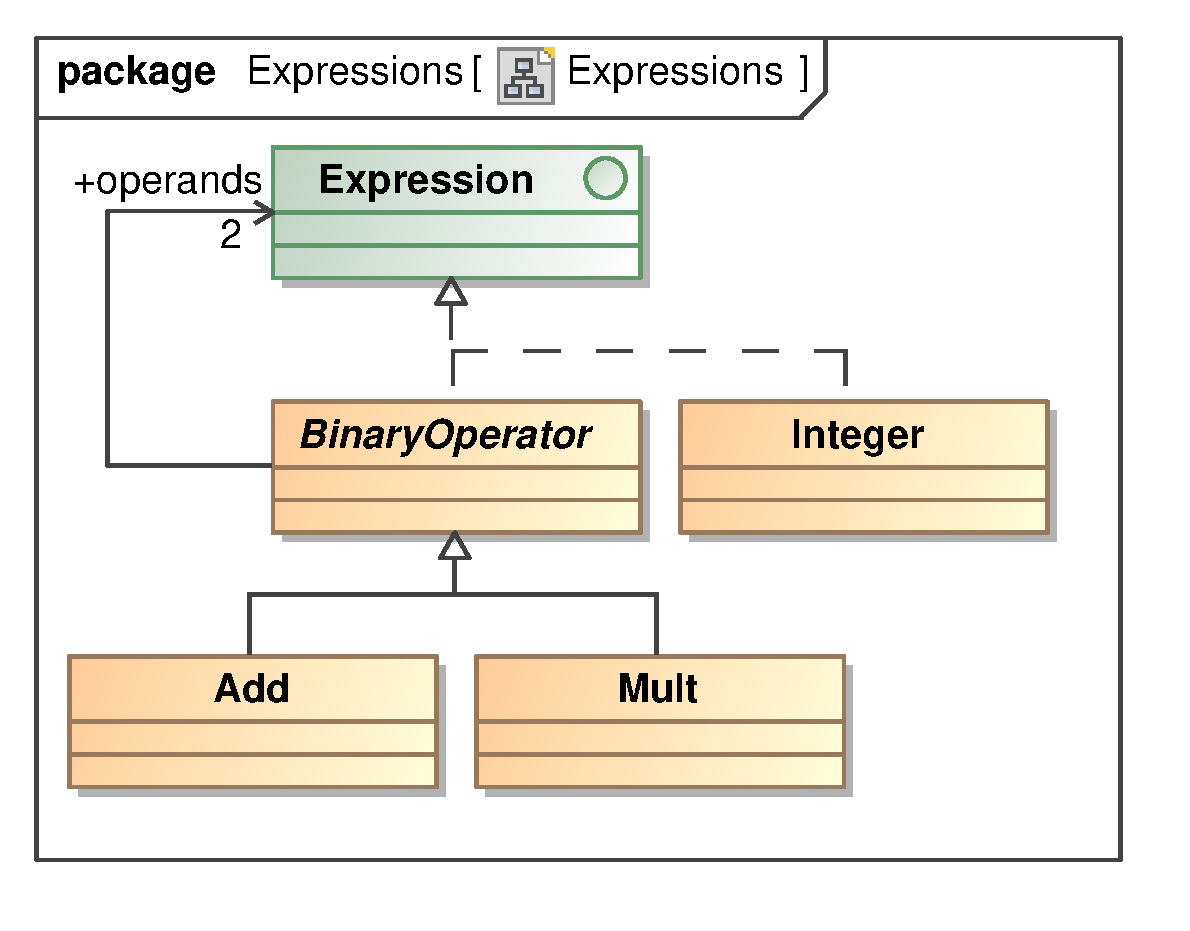
\includegraphics[width=.60\linewidth]{background/images/Expressions.eps} \\
  \caption{Diagrama de clases para el problema de las expresiones}
  \label{back:fig:expr}
\end{figure}
\begin{figure}[ht!]
  % Requires \usepackage{graphicx}
  \centering 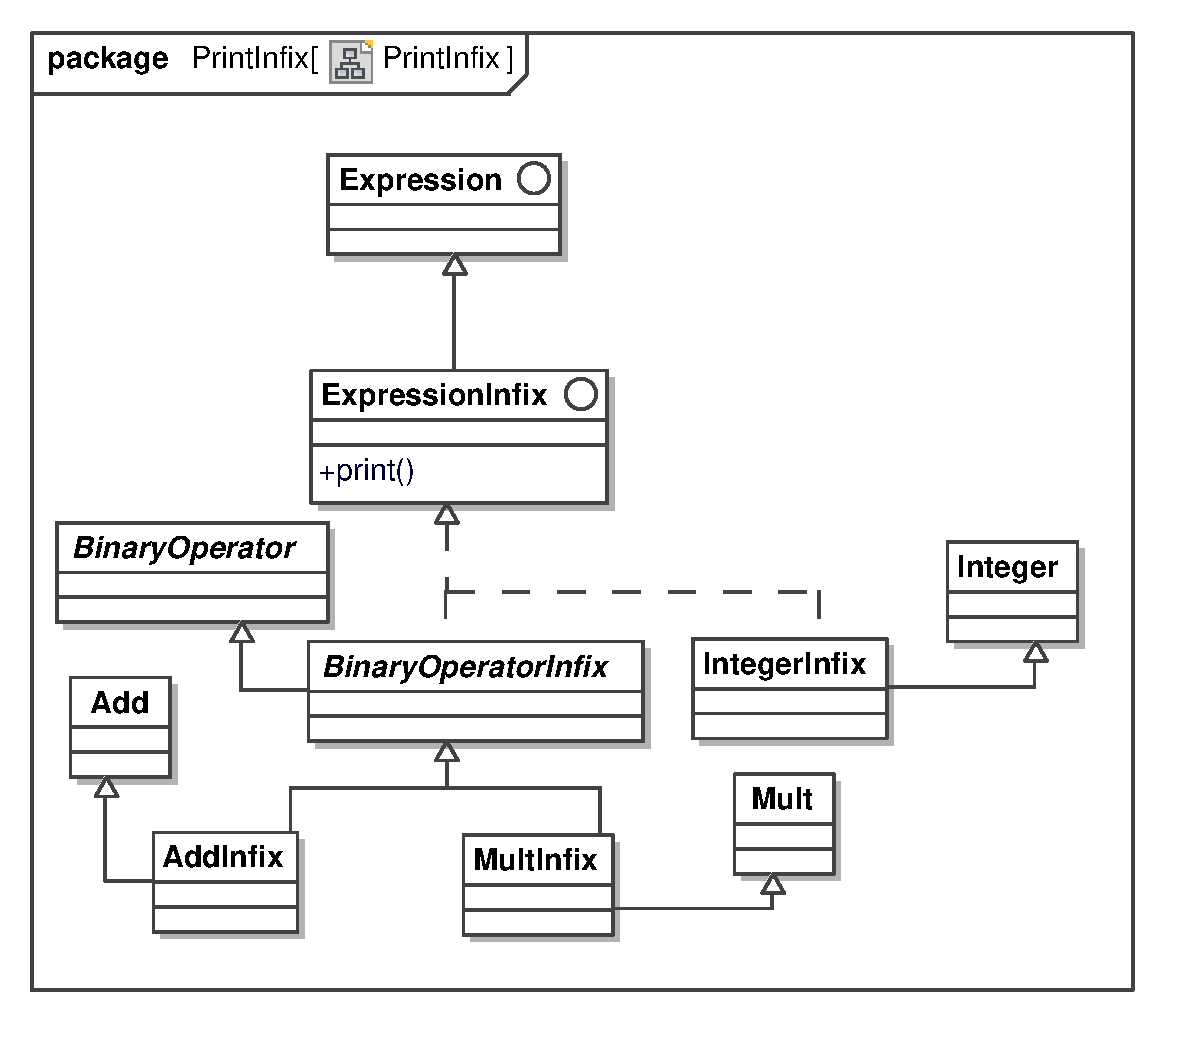
\includegraphics[width=.80\linewidth]{background/images/PrintInfix.eps} \\
  \caption{Diagrama de clases para la operaci�n de imprimir en formato infijo}
  \label{back:fig:printInfix}
\end{figure}
Tras trasladar estos diagramas a C\# se observan las carencias que posee un lenguaje orientado a objetos cuando implementamos un problema propio de la programaci�n orientada a caracter�sticas.\\
Por un lado he utilizado el mecanismo de herencia para a�adir funcionalidades a una clase existente, pero este mecanismo es jer�rquico, lo que hace que la clase hija herede toda la funcionalidad de su clase padre.
Por ejemplo, para crear una nueva configuraci�n que contenga las operaciones evaluar e imprimir en formato infijo se necesitar�a crear una nueva subclase que heredase de las clases que contienen las operaciones citadas anteriormente, pero esto no es posible, ya que C\#, como la mayor�a de los lenguajes orientados a objetos, solo permiten hacer uso de la herencia m�ltiple entre interfaces. Por lo tanto, por cada clase que se quiera heredar debemos crear una nueva interfaz que sea extendida por la clase a heredar y por la subclase que contendr� la nueva configuraci�n, a trav�s de esto y la creaci�n de objetos de las clases a heredar podremos acceder a los m�todos definidos por las interfaces, con lo que se consigue simular la herencia m�ltiple.\\
Pero el uso de esta t�cnica hace que, un incremento de funcionalidad representado por un conjunto de nuevas subclases que heredan de un conjunto de clases superiores, no sea posible manejarlo consistentemente como una unidad encapsulada. La insuficiente unidad de encapsulaci�n, deriva en un problema de complejidad en el manejo de la selecci�n de caracter�sticas para la composici�n. Aun cuando, las clases separadas en paquetes pertenezcan a una misma caracter�stica, es necesario seleccionar clases concretas que van a ser usadas en un producto espec�fico.
Otro problema es el manejo de las dependencias, ya que la herencia tradicional obliga a que las clases y subclases tengan diferentes nombres. Por lo tanto, las referencias a las clases concretas deben ser actualizadas. A mayor n�mero de caracter�sticas en una l�nea de productos, las relaciones entre clases concretas se complican potencialmente, lo que resulta una situaci�n indeseable. Esto incrementa la complejidad en las relaciones y dependencias entre clases.
% - Cuentas el ejemplo de las expresiones
% - Muestras la soluci�n en C#.

\subsubsection{Conclusiones}

Tras analizar el problema con un lenguaje orientado a objetos como es C\# se podr�a determinar que ser�a deseable encontrar en un lenguaje de programaci�n que estuviese orientado a caracter�sticas para obtener f�cilmente diferentes versiones de una misma aplicaci�n con la simple combinaci�n de diferentes conjuntos de caracter�sticas. Obviamente no todas las combinaciones ser�n v�lidas, por lo tanto, un lenguaje orientado a caracter�sticas deber�a de intentar asegurarse de que el resultado de la composici�n produce una aplicaci�n segura y bien configurada.
Con lo citado anteriormente, vamos a identificar una serie de caracter�sticas deseables que deber�amos encontrar en un lenguaje orientado a caracter�sticas:\\\\
\emph{Extensibilidad a trav�s de la adici�n y la substituci�n}\\
Como ya hemos comentado, una caracter�stica es normalmente considerada como un incremento en la funcionalidad de un programa. Por lo tanto, los lenguajes orientados a caracter�sticas deben proveer mecanismos para a�adir nuevas funcionalidades a una existente. En los lenguajes orientados a objetos, la extensi�n es realizada a trav�s de la herencia, pero �sta es adecuada cuando queremos extender una sola clase, pero com�nmente, las caracter�sticas necesitan ser extendidas por varias clases al mismo tiempo.
Adem�s la extensibilidad no siempre se alcanza por adici�n, en ocasiones es necesario el uso de la substituci�n. En los lenguajes orientados a objetos la substituci�n es llevada a trav�s de m�todos de sobre escritura (override en ingl�s).\\\\
\emph{Encapsulaci�n de caracter�sticas}\\
Todas las extensiones pertenecientes a una caracter�stica concreta deben ser a�adidas de una forma at�mica. Por lo tanto, los lenguajes orientados a caracter�sticas deber�an proveer de mecanismo para agrupar y encapsular los m�dulos pertenecientes a una misma caracter�stica. Por otra parte, estos m�dulos deber�an poderse compilar independientemente.\\\\
\emph{Composici�n a nivel de caracter�stica}\\
Productos espec�ficos, o configuraciones de una descomposici�n orientada a caracter�sticas, son obtenidos por la selecci�n y composici�n de unas caracter�sticas espec�ficas. Por lo tanto, ser�a deseable que un lenguaje orientado a caracter�sticas tuviese construcciones del lenguaje para producir un producto en particular. Esto deber�a ser realizado a nivel de caracter�stica, especificando que caracter�sticas deber�an ser incluidas, en lugar de tener que especificar los elementos individuales de cada caracter�stica.\\\\\\
\emph{Composici�n de caracter�sticas comprobando la coherencia}\\
No todas las combinaciones de caracter�sticas son v�lidas. Por lo tanto, un lenguaje orientado a caracter�sticas deber�a detectar las restricciones, evitando as� la implementaci�n de configuraciones no v�lidas y manejar autom�ticamente las dependencias en la medida de lo posible.

\subsection{Ventajas de los lenguajes orientados a caracter�sticas}
Los lenguajes orientados a caracter�sticas nos otorgan una mayor flexibilidad, ya que nos permiten que clases individuales puedan ser compuestas por un conjunto de caracter�sticas, por tanto son especialmente recomendados para utilizarlos con las l�neas de producci�n software.\\
Para estudiar las ventajas de los lenguajes orientados a caracter�sticas se trabajar� con CaesarJ que es un lenguaje de programaci�n basado en Java, que nos proporciona una mayor modularidad y el desarrollo a trav�s de componentes reusables.Para ello trabaja con conceptos como clases y paquetes en una �nica entidad, llamada familia de clases, que constituye unidades de encapsulamiento adicional para agrupar clases relacionadas. Una familia de clases tambi�n es, en s� misma una clase. As� mismo, se introduce el concepto de clases virtuales, que son clases internas (de familias de clases) propensas a ser refinadas a nivel de subclases. En el refinamiento de una clase virtual, impl�citamente se hereda de la clase que refina, por lo que tambi�n esto es visto como una relaci�n adjunta. Tambi�n, en un refinamiento pueden ser a�adidos nuevos m�todos, campos, relaciones de herencia y sobreescritura de m�todos. Puesto que en cada familia de clases, las referencias a las clases virtuales siempre apuntar�n al refinamiento m�s espec�fico. Esto significa que, por medio de las clases virtuales se aplica sobre escritura de m�todos, permitiendo redefinir el comportamiento de cualquier subclase de una familia de clases.\\
En t�rminos de programaci�n orientada a caracter�sticas, cada funcionalidad es modelada como una familia de clases. Mientras que los componentes y objetos del dominio espec�fico, son correspondidos por sus clases virtuales. As� mismo, las clases virtuales pueden ser declaradas como clases abstractas, lo que habilita la definici�n de interfaces en la implementaci�n modular de caracter�sticas.\\\\
Para hacer uso de lo citado anteriormente y ver su beneficio con las l�neas de producci�n software se ha vuelto a utilizar el ya comentado problema de las expresiones de la subsecci�n anterior. Pero en este caso, el dise�o cambia significativamente debido a la caracter�sticas expuestas de CaesarJ.\\
Por un lado en la figura \ref{back:fig:caesarJExpressions} se muestra que por cada operaci�n, tenemos una familia de clases, siendo la familia de clases que encapsula a todas las dem�s, la denominada \imp{Expressions}. �sta tiene la estructura de clases representado en la figura \ref{back:fig:expr}, y cada familia de clases lo que hace es redefinir las clases virtuales de \imp{Expressions} con las operaciones necesarias en cada caso.\\
\begin{figure}[ht!]
  % Requires \usepackage{graphicx}
  \centering 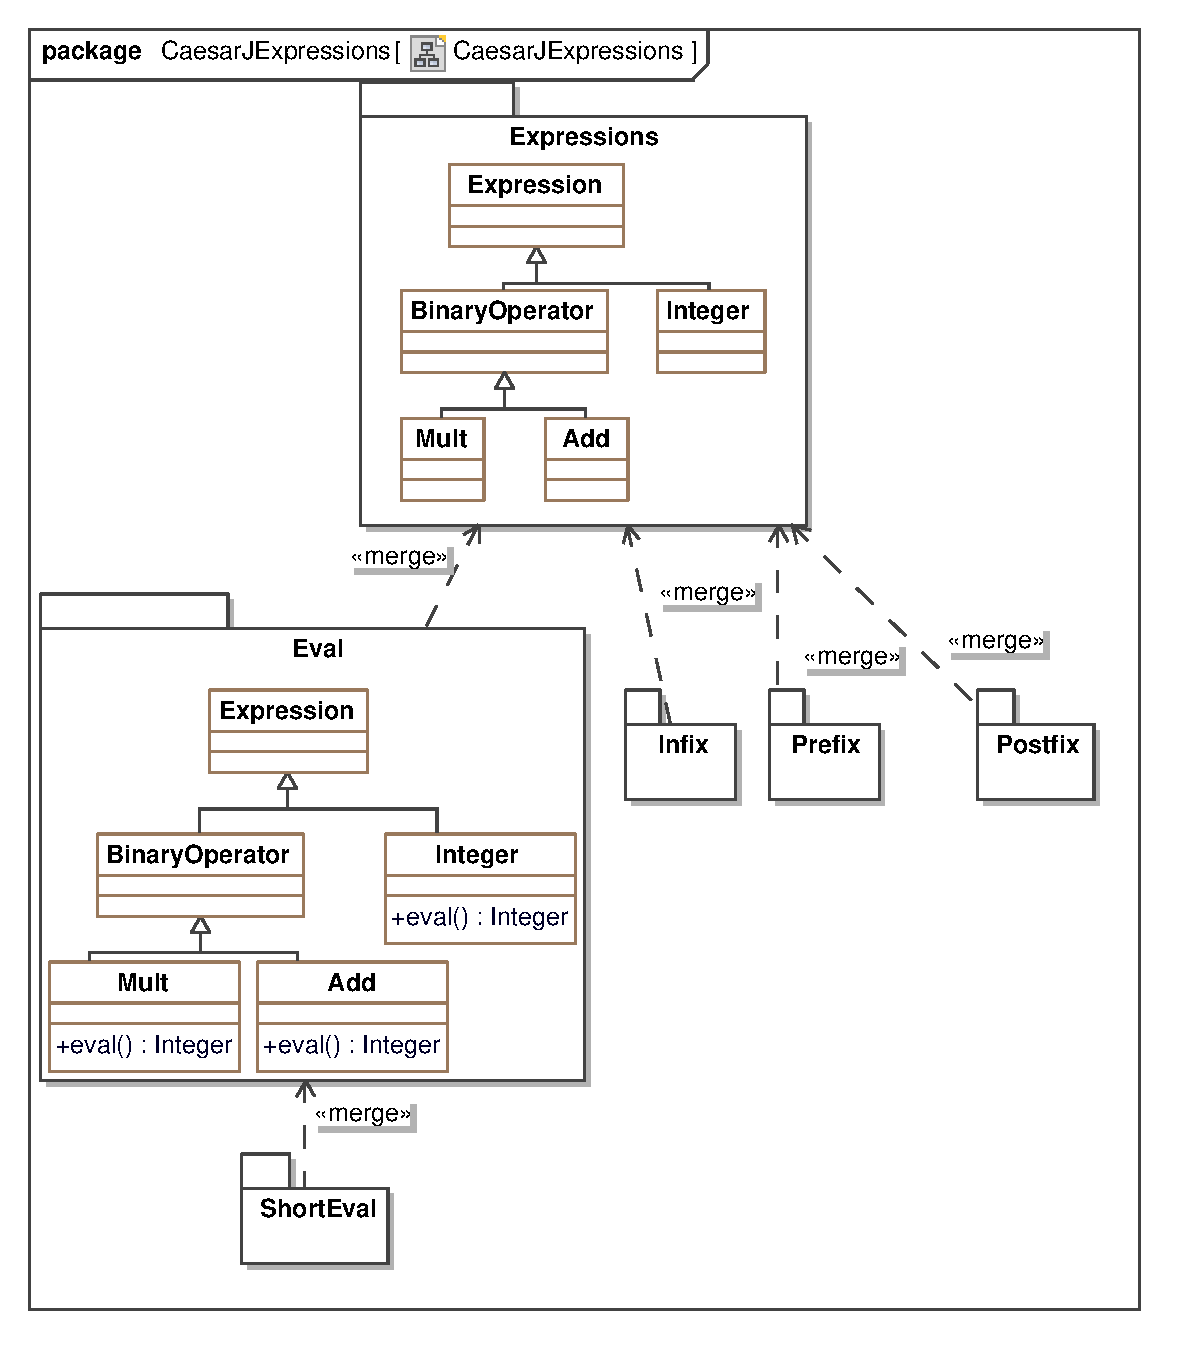
\includegraphics[width=.60\linewidth]{background/images/CaesarJExpressions.eps} \\
  \caption{Dise�o para resolver el problema de las expresiones con CaesarJ}
  \label{back:fig:caesarJExpressions}
\end{figure} 
\begin{figure}[ht!]
\begin{center}
\begin{footnotesize}
\begin{verbatim}
00 import eval.Eval;
01 import printPostfix.PrintPostfix;
02 import printInfix.PrintInfix;
03 import printPrefix.PrintPrefix;
04 public cclass EvalInfix extends PrintPrefix & Eval {}
\end{verbatim}
\end{footnotesize}
\end{center}
\caption{Configuraci�n que incluye las operaciones de evaluar e imprimir en formato infijo con CaesarJ}
\label{back:fig:codCaesarJ}
\end{figure}

Para realizar configuraciones, �nicamente se tiene que crear una nueva clase que extienda a las caracter�sticas que se deseen.A modo de ejemplo,la figura \ref{back:fig:codCaesarJ} muestra el c�digo necesario para crear una nueva configuraci�n que contenga las operaciones de impresi�n en formato posfijo y evaluaci�n de una expresi�n.Con todo esto, vemos como CaesarJ otorga un gran nivel de encapsulamiento y de reusabilidad de los componentes.

% P�rrafo introducci�n
% Introducci�n CaesarJ
% Ejemplo en CeasrJ, resaltando ventajas

\section{Clases Parciales C\#}
Las clases parciales C\# \cite{albahari:2010} nos permiten dividir la implementaci�n de una clase, estructura o interfaz en varios archivos de c�digo fuente. Cada fragmento representa una parte de la funcionalidad global de la clase. Todos estos fragmentos se combinan en tiempo de compilaci�n para crear una �nica clase, la cual contiene toda la funcionalidad especificada en las clases parciales. Por lo tanto,las clases parciales C\# pueden utilizarse como un mecanismo adecuado para implementar caracter�sticas, dado que cada incremento en funcionalidad para una clase se podr�a encapsular en una clase parcial separada.\\\\
Para poder ser compiladas y agrupadas en una sola clase, todas las clases parciales deben pertenecer al mismo espacio de nombres, poseer la misma visibilidad y deben ser declaradas con el indicador clave partial. En C\#, un espacio de nombre es simplemente empleado para agrupar clases relacionadas y evitar conflictos de nombres. Para especificar los archivos C\# que deben ser incluidos en una compilaci�n, se emplea un documento XML que contiene informaci�n acerca del proyecto y que especifica que ficheros deben ser compilados para generar el proyecto. Por lo tanto, es posible incluir y excluir f�cilmente la funcionalidad encapsulada dentro de una clase parcial simplemente a�adiendo o eliminando dicha clase parcial de este fichero XML.\\\\
Para ilustrar lo dicho anteriormente, se ha vuelto a utilizar el problema de las expresiones implement�ndolo con clases parciales. La figura \ref{back:fig:partialClass} muestra como hemos excluido de la compilaci�n la caracter�stica que representa la operaci�n de imprimir una expresi�n en formato infijo.
Este mecanismo de clases parciales permite a�adir o compartir funcionalidad entre un conjunto de clases que no precisan estar relacionadas mediante ning�n tipo de relaci�n jer�rquica, tal como ocurre con la herencia.\\
Por lo tanto, algunos autores (Laguna et al, 2007) sostienen que, las clases parciales C\# representan una alternativa a la herencia m�ltiple para manejar variabilidad relacionada programaci�n orientada a caracter�sticas.
\begin{figure}[!t]
\begin{center}
\begin{footnotesize}
\begin{verbatim}
01    <itemgroup>
02    <!--Eval-->
03    <Compile Include="Eval\Add.cs" />
04    <Compile Include="Eval\IExpressionsEval.cs" />
05    <Compile Include="Eval\IExpressions.cs" />
06    <Compile Include="Eval\Integer.cs" />
07    <Compile Include="Eval\Mult.cs" />
08    <!--Infix-->
09    <!--<Compile Include="Infix\Add.cs" />
10    <Compile Include="Infix\IExpressionInfix.cs" />
11    <Compile Include="Infix\IExpressions.cs" />
12    <Compile Include="Infix\Integer.cs" />
13    <Compile Include="Infix\Mult.cs" />-->
14    ...
15    </itemgroup>
16    </Project>
\end{verbatim}
\end{footnotesize}
\end{center}
\caption{Implementaci�n del archivo XML que guarda la informaci�n para la compilaci�n}
\label{back:fig:partialClass}
\end{figure}

% Qu� hace esto aqu�

% Explicar que son brevemente, y ejemplo usando las expresiones



% Cap�tulo 3: Domain Engineering
% %%==================================================================%%
%% Author : Abascal Fern�ndez, Patricia                             %%
%% Author : S�nchez Barreiro, Pablo                                 %%
%% Version: 1.2, 24/06/2013                                         %%
%%                                                                  %%
%% Memoria del Proyecto Fin de Carrera                              %%
%% Application Engineering/Introduccion                             %%
%%==================================================================%%

Este cap�tulo describe el proceso de desarrollo de los generadores de c�digo para la segunda fase del desarrollo de una l�nea de productos software (ver Figura~\ref{back:fig:domainAplicEng}), el proceso de \emph{Ingenier�a de Aplicaciones}. El objetivo de esta fase, tal como comentamos, es obtener productos concretos y funcionales a partir de la composici�n, configuraci�n y personalizaci�n de los elementos creados en la fase de \emph{Ingenier�a del Dominio}.

Para ello, de acuerdo con la metodolog�a Te.Net (ver Secci�n~\ref{sec:intr:tenet}), el primer paso es crear una selecci�n de aquellas caracter�sticas que se desea incluir en el producto, de acuerdo a las necesidades particulares de cada cliente. C�mo se crea dicha selecci�n de caracter�sticas est� fuera del �mbito de este proyecto. Referimos al lector interesado al Proyecto Fin de Carrera de D. Daniel Tejedo, antiguo alumno de esta Facultad~\citep{daniel:2013}.

Una vez obtenida una selecci�n de caracter�sticas v�lida, utilizando dicha selecci�n, se configura la arquitectura de referencia creada en la fase de \emph{Ingenier�a del Dominio} para crear un modelo arquitect�nico concreto, adaptado a las necesidades del cliente, del producto que queremos construir.  Dicho modelo arquitect�nico se obtiene de forma autom�tica mediante la utilizaci�n del lenguaje \emph{VML}~\citep{loughran:2008,sanchez:2008}, de acuerdo con la metodolog�a Te.Net (ver Secci�n~\ref{sec:intr:tenet}). Una descripci�n detallada del lenguaje VML tambi�n est� fuera del �mbito de este proyecto, y referimos al lector interesado al trabajo de~\cite{daniel:2013}.

Este modelo arquitect�nico de un product concreto es el que sirve de entrada al generador de c�digo que queremos desarrollar. Utilizando dicho modelo como entrada, el generador de c�digo debe producir todo el c�digo necesario para componer las clases parciales creadas a nivel de \emph{Ingenier�a del Dominio} que correspondan. Para ello debe generar las clases parciales encargadas de llevar a cabo tal composici�n, las versiones limpias de los m�todos requeridos, y las delegaciones a las versiones sucias adecuadas.

Para ello, el primer paso era dise�ar un algoritmo que permitiese calcular estos tres elementos: (1) clases parciales requeridas; (2) versiones limpias necesarias; y, (3) delegaciones adecuadas. A continuaci�n, deb�amos implementar este algoritmo utilizando plantillas de generaci�n de c�digo, por lo que deb�amos, igual que en cap�tulo anterior, prestar especial atenci�n a su secuenciaci�n.

Por �ltimo, deb�amos dise�ar y realizar las pruebas que permitiesen comprobar el correcto funcionamiento del generador de c�digo. Tras estas pruebas, se daba por concluido el proceso de desarrollo de los generadores de c�digo, y procedimos a su despliegue.

Para explicar este proceso de desarrollo, este Cap�tulo se estructura como sigue: La Secci�n~\ref{application:sec:alg} describe la estructura de los modelos de entrada que nuestro generador de c�digo debe procesar. La Secci�n~\ref{application:sec:alg} describe el dise�o del algoritmo encargado de calcular los elementos a componer, de acuerdo al modelo de entrada proporcionado. La Secci�n~\ref{application:sec:transf} explica c�mo se han secuenciado las plantillas de generaci�n de c�digo para poder implementar dicho algoritmo. La Secci�n~\ref{application:sec:pruebas} describe el proceso de dise�o y ejecuci�n de las pruebas para el generador de c�digo implementado. Por �ltimo, la Secci�n~\ref{application:sec:despliegue} detalla las acciones realizadas durante la fase de despliegue de la aplicaci�n.








% Cap�tulo 6: Discusi�n, Conclusiones y Trabajos Futuros
% \todo{Cap�tulo 7: Discusi�n, Conclusiones y Trabajos Futuros}

% CONTENT: Appendices, if desired
% \appendix
\chapter{Descripci�n de los contenidos del CD adjunto}

 A continuaci�n se describen la ubicaci�n y el contenido del CD adjunto a esta memoria:
 \begin{enumerate}
 \item En la carpeta Instaladores se encuentran los dos plugins desarrollados durante este proyecto.
 \item En la carpeta Documentos/Manuales se encuentran disponibles los distintos manuales creados\footnote{Los manuales tambi�n se encuentran disponibles en la URL http://www.alumnos.unican.es/apr85/.}.
 
 \end{enumerate}


% Appendix A:
% \input{populo/populo.tex} % Appendix I

% CONFIG: Bibliography style
%\cleardoublepage                            % start in right side page
\addcontentsline{toc}{chapter}{Referencias}  % add this "chapter" to the ToC, with the name "Bibliography"
%pohl:2005\bibliographystyle{alpha}                  % bibliography style
%clements:2002\bibliographystyle{alpha}
%batory:2004\bibliographystyle{alpha}
%albahari:2010\bibliographystyle{alpha}
%\bibliographystyle{abbrv}                  % bibliography style
\bibliographystyle{alpha}

\bibliography{references/references}

\end{document}
